% !TeX root = RJwrapper.tex
\title{An Empirical Exploration of the Vibrant R Ecosystem}
\author{by Tian-Yuan Huang and Liying Yang}

\maketitle

\abstract{%
Created in the late 20th century, R is one of the most popular software
environments for statistical computing and graphics. Embracing the
development of information technology and the advent of the big data
era, great changes have taken place in the R ecosystem during recent
years. An empirical review is carried out based on meta-information of
CRAN and bibliometric data of the literature citing R. We discovered
that while initiated by statistics, the development of R benefited
greatly from software developers and users coming from various
disciplines such as agricultural, biological, environmental, and medical
science. In addition, we show the collaboration patterns among R
developers and analyze the possible effects of collaboration in the R
community. By exploring the R ecosystem and making critical discussions,
we intend to gain a better understanding of the current R ecosystem and
provide a reference for the ecosystem's future development.
}

\hypertarget{introduction}{%
\section{Introduction}\label{introduction}}

Among the various programming languages, R is famous for its capability
in data mining. Yet, the TIOBE Index for programming languages has found
a decreasing trend in the use of R from 2018 to 2019
(\url{https://www.tiobe.com/tiobe-index/r/}). While few people dig into
the details of how this index is calculated, this popular index did
bring panic and depressed some R users and developers, even those who
had been using R for years. But according to the download logs of CRAN
(the Comprehensive R Archive Network), neither R software nor R packages
are facing a reduction in the downloads during this period (Figure 1).
On the contrary, there was a remarkable leap in the latter half of 2018.
The data shows that August 2018 was the tipping point for the number of
downloads (at monthly level), both for R software and R packages. There
is no doubt that R has been used by more people and more frequently over
time.

As a programming language, R's free open-source environment was derived
from the S language, developed at Bell Labs during the seventies. The R
core was first launched in 1997 and is maintained by the R Core Team and
R Foundation since then. The public management of R packages is mainly
supported by CRAN, while other major repositories include BioConductor,
R-Forge, and GitHub \citep{GermanAdams-562, PlakidasSchall-561}. While
these repositories have overlapping packages, CRAN remains the center of
the R package management system \citep{DecanMens-557}. The usage of R is
extensive and gradually R has become one of the most popular softwares
in scientific research. This has led scientists to pay more attention to
the scientific usage of R packages. Related investigations focus on the
co-mentioning network of R packages \citep{LiYan-560} and citation
patterns of specific or general R packages
\citep{LiChen-558, LiYan-559}. In addition, numerous studies have shown
that researchers and practitioners from various backgrounds embrace R
for its openness and reproducibility
\citep{GentlemanCarey-499, PebesmaNst-498, HuberCarey-496, LowndesBest-495, KayaAgca-491, LaiLortie-492},
though creating and maintaining software itself is not generally
recognized as an academic accomplishment \citep{YangRousseau}.

In this paper, we would like to suggest a new framework for the R
ecosystem and provide an empirical review of it based on the metadata
from CRAN (\url{https://cran.r-project.org/}) and Scopus, the well-known
database provided by Elsevier (\url{https://www.scopus.com/}). The
concept of a software ecosystem was first suggested around 2000
\citep{MesserschmittSzyperski-609}, and developed rapidly in the
following years
\citep{IansitiLevien-615, Hanssen-614, ManikasHansen-611, Jansen-613}.
By drawing upon the well-established concept of an ``ecosystem'' in
ecology, this approach tries to classify members into different
components, investigate their characteristics, and study their
interactions. In this way community members from possibly segregated
sections benefit by seeing how they are part of the whole. Extending
this concept to the open-source software community, research on open
source ecosystems has been carried out for various programming
languages, including Ruby \citep{KabbedijkJansen-623, SyeedHansen-624},
Python \citep{HovingSlot-617}, and R
\citep{GermanAdams-562, PlakidasSchall-561, DecanMens-557}.

Previous studies suggest that the R ecosystem consists of three main
areas, namely the R platform, the software marketplace(s), and the
community \citep{PlakidasSchall-561}. Inspired by this framework, we
provide some adjustments and extensions to make the software ecosystem
more similar to a biological ecosystem. The proposed framework for the R
ecosystem is displayed in Figure 2. Software developers act as producers
of the ecosystem, they build tools and provide products (e.g., R
packages) for the users (considered as consumers). General users have
various demands for the statistical designers (considered as
decomposers) according to their tasks. Then, the statistical designers
propose multiple algorithms to meet the needs of the users, and the
required algorithms are then transferred to the software developers to
make better products. In addition, the developers must provide a
software platform for the statistical designers, so that they can test
their ideas and schemes. While these three groups of members may
overlap, abstracting these roles helps us understand different driving
models of the development of the R ecosystem. Based on this framework,
we explore four specific questions from different perspectives.

\begin{enumerate}
\def\labelenumi{\arabic{enumi}.}
\tightlist
\item
  From the perspective of software developers: what are the most popular
  R packages over the late 15 years since 2005 and why?
\item
  From the perspective of academic users: which fields do they come from
  and why are they using R?
\item
  From the perspective of statistical designers: what motivate them to
  develop R packages?
\item
  From the perspective of the global R community: How do they
  collaborate and to what extent?
\end{enumerate}

By exploring these questions and making critical discussions, we intend
to gain a better understanding of the current R ecosystem and shape the
future development of R.

\begin{Schunk}
\begin{figure}
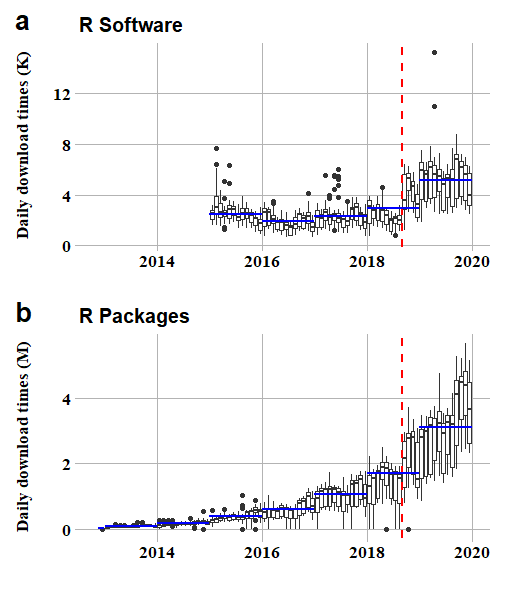
\includegraphics[width=1\linewidth,height=0.3\textheight]{fig1} \caption[The daily downloads of R software (a) and R packages (b)]{The daily downloads of R software (a) and R packages (b). The boxplots show the daily number of downloads in a month. The blue lines show the average daily download in each year, and the dashed red line indicates where the number of downloads shows a sudden change (yielded by changepoint package). Source of data: http://cran-logs.rstudio.com/. }\label{fig:fig1}
\end{figure}
\end{Schunk}

\begin{Schunk}
\begin{figure}
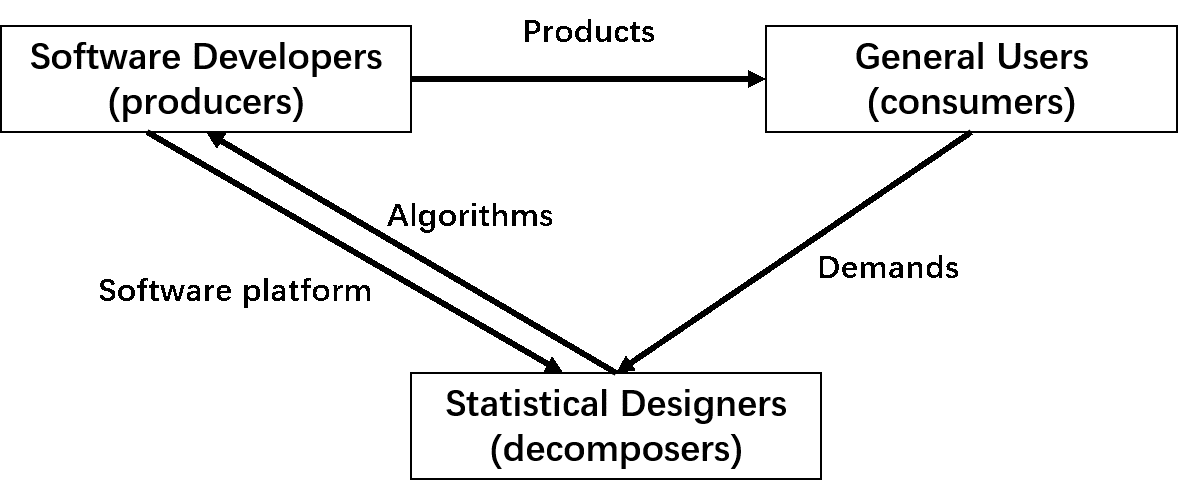
\includegraphics[width=1\linewidth,height=0.3\textheight]{fig2} \caption[Framework of the R ecosystem in our study]{Framework of the R ecosystem in our study. This resembles the biological ecosystem which consists of three main roles, namely producers, consumers, and decomposers. }\label{fig:fig2}
\end{figure}
\end{Schunk}

\hypertarget{data-and-software}{%
\section{Data and software}\label{data-and-software}}

To get a comprehensive view of the R ecosystem, multiple data sources
are collected and utilized, namely (1) Download information of R and R
packages. These download logs were accessed from Rstudio CRAN Mirror
(\url{http://cran-logs.rstudio.com/}), and information on the daily
number of downloads was retrieved via APIs from \CRANpkg{cranlogs}
package; (2) Metadata of R packages on CRAN. The metadata of R packages,
such as their authors, maintainers, published date and imported packages
(dependent packages),are archived in CRAN. These data were extracted
using \CRANpkg{RWsearch} package. The target data in our research was
retrieved on January 1st, 2020; (3) Bibliometric data of papers citing
R: The bibliometric data could helped us to explore how R is utilized in
academia. Referring to the previous research \citep{LiYan-559}, our
study retrieved the bibliometric data of papers citing R software from
Scopus using advanced search (the advanced query was ``REF (\{R: A
Language and Environment for Statistical Computing\} OR
\{\url{http://www.r-project.org}\}) AND DOCTYPE (ar)''), yielding
364,928 articles published from 2005 to 2019. The \CRANpkg{rscopus}
package was used to facilitate the acquisition of bibliometric data from
Scopus. The bibliometric data contains information of publication year,
title, keywords, journal title, ISSN, etc. Scopus Subject Area
categories were used to classify the publications into different
subjects. The data analyses were carried out in R software. The R
packages used in the study include \CRANpkg{tidyverse},
\CRANpkg{data.table}, \CRANpkg{patchwork}, \CRANpkg{changepoint},
\CRANpkg{lubridate}, \CRANpkg{fst}, \CRANpkg{akc},
\CRANpkg{graphlayouts} and \CRANpkg{tidyfst}.

\hypertarget{method-and-results}{%
\section{Method and results}\label{method-and-results}}

\hypertarget{popular-r-packages}{%
\subsection{Popular R packages}\label{popular-r-packages}}

Examining the most downloaded R packages in total on CRAN between 2005
and 2019, we found that the top 10 R packages (Figure 3a) have a share
of about 10\% of the total downloads. These packages provide essential
functionalities for further development in the R ecosystem. Among them,
\CRANpkg{ggplot2}, \CRANpkg{stringr} (a wrapper of \CRANpkg{stringi}),
\CRANpkg{dplyr} might be the best known to end-users because they are
completely data-oriented and easy to use with consistent and readable
APIs. Furthermore, packages like \CRANpkg{Rcpp}, \CRANpkg{digest},
\CRANpkg{rlang} and \CRANpkg{R6} brought great convenience to R
programmers (especially software developers), and thus are often
imported by other packages during R development. Especially,
\CRANpkg{magrittr} and \CRANpkg{tibble}, add fundamental functionalities
to other packages. Simply representing ``and then'' in natural language,
the operator \texttt{\%\textgreater{}\%} in \CRANpkg{magrittr} is
elementary for R as a language. This implementation is in line with the
logic of human thinking. It reduces development time and improves the
readability and maintainability of R code. As the pipe syntax has gained
recognition and acceptance, on May 18, 2021, a native pipe
(\texttt{\textbar{}\textgreater{}}) was introduced in the released R
version 4.1.0. Moreover, considering R as an environment, ``data frame''
is an important data structure (a two-dimension table with rows and
columns), and \CRANpkg{tibble} has offered an enhanced class (named
`tibble' or `tbl\_df') for it. This redesigned class provides end-users
the means to inspect the traditional data frame fast and safely.
Therefore, it is adopted by many other R packages and widely used in
data science workflows, especially for big data analysis.

Turning to the list of monthly downloads (Figure 3b), we see more
packages designed for R developers are releasing, including
\CRANpkg{pillar}, \CRANpkg{lifecycle}, \CRANpkg{cli} and
\CRANpkg{fansi}. As a complementary component to string operation,
\CRANpkg{glue} is also gaining popularity and becomes the main package
imported in other utilities (including \CRANpkg{stringr}). Finally, as
part of the ``cloudyr'' project (\url{https://cloudyr.github.io/}), the
rise of the \CRANpkg{aws.s3} and the \CRANpkg{aws.ec2metadata} package
has revealed another trend, namely using and developing R in a cloud
computing platform. To conclude, the popularity of modern R mainly
depends on software facilities provided by the R environment, which
greatly improves the reliability and efficiency of data science
workflows.

\begin{Schunk}
\begin{figure}
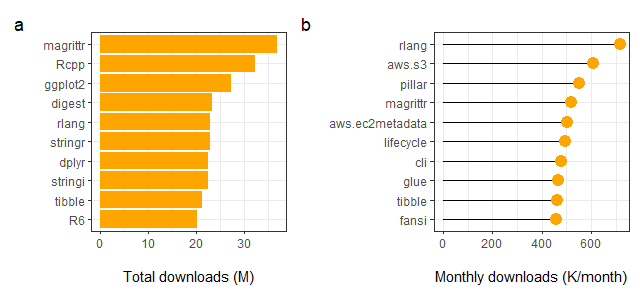
\includegraphics[width=1\linewidth,height=0.3\textheight]{fig3} \caption[Top 10 R packages (a) by total downloads and (b) by monthly downloads from 2005 to 2019 since publication]{Top 10 R packages (a) by total downloads and (b) by monthly downloads from 2005 to 2019 since publication. }\label{fig:fig3}
\end{figure}
\end{Schunk}

\hypertarget{applications-of-r-in-academia}{%
\subsection{Applications of R in
academia}\label{applications-of-r-in-academia}}

According to Scopus, the number of academic articles citing R software
has been steadily increasing from 2005 to 2019 (Figure 4a). While only
1057 citations were tracked in 2005, the number of articles citing the R
software has reached a total of 62,168 citations in 2019. Considering
the subject area of these articles, we found a remarkable upward trend
of R usage in ``Agricultural and Biological Sciences'', ``Biochemistry,
Genetics, and Molecular Biology'', ``Earth and Planetary Sciences'',
``Environmental Science'', ``Immunology and Microbiology'',
``Medicine'', ``Psychology'' and ``Social Sciences'' (Figure 4b). This
is probably due to the flourishing of measurement methods and data
sciences in these scientific fields. During this period of 15 years
``Agricultural and Biological Sciences'' and ``Environmental Science''
turned out to be the most active subject areas using R (Figure 4c and
Figure 4d). Not only did they publish most articles based on R (106,853
and 51,522 respectively), but they also had the highest percentage of
articles utilizing R (4.5\% and 3.3\% respectively). Although,
intuitively, ``Computer Science'' and ``Mathematics'' should be
considered most relevant to R, they had a relatively low number of
articles citing R. From 2005 to 2019, there were 10,111 articles
categorized as ``Mathematics'' citing R (0.7\% within the subject area),
whereas in ``Computer Science'' there were only 7,164 articles citing R
(0.5\% within the subject area).

\begin{Schunk}
\begin{figure}
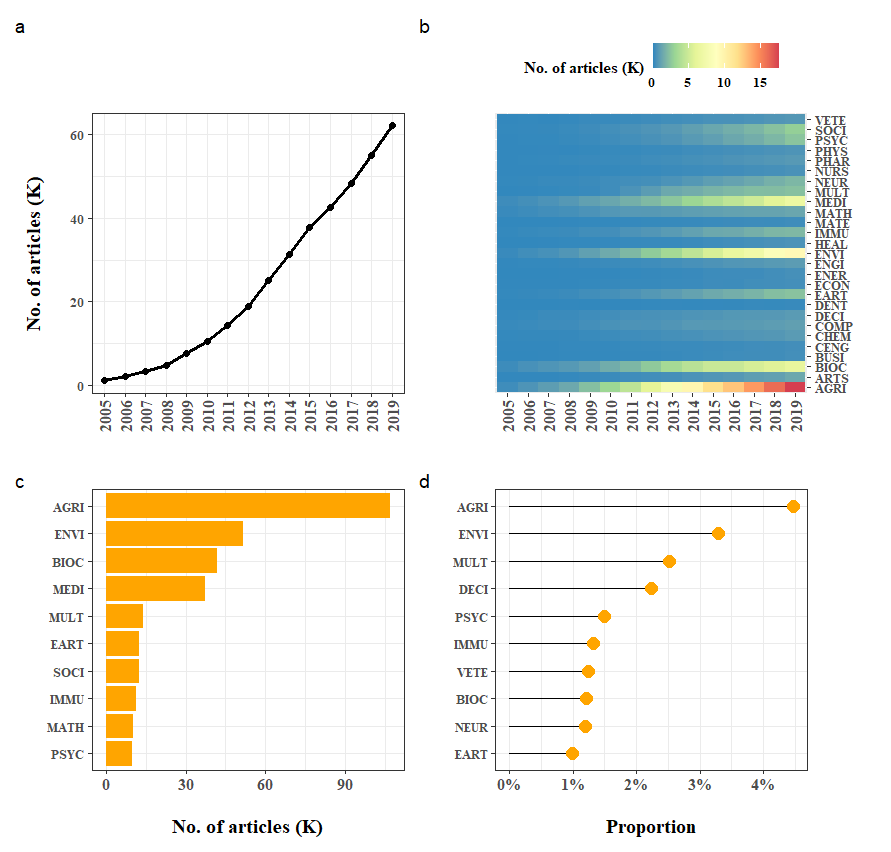
\includegraphics[width=1\linewidth,height=0.3\textheight]{fig4} \caption[Usage of R in academia between 2005 and 2019]{Usage of R in academia between 2005 and 2019. (a) Growth of academic articles citing R software. (b) The number of articles citing R software in different subject areas over time. (c) Top 10 subjects with most articles citing R software. (d) Top 10 subjects with the largest proportion of articles citing R software. The subject classification is based on the list of Scopus Subject Area (AGRI: Agricultural and Biological Sciences; ARTS: Arts and Humanities; BIOC: Biochemistry, Genetics, and Molecular Biology; BUSI: Business, Management, and accounting; CENG: Chemical Engineering; CHEM: Chemistry; COMP: Computer Science; DECI: Decision Sciences; DENT: Dentistry; EART: Earth and Planetary Sciences; ECON: Economics, Econometrics, and Finance; ENER: Energy; ENGI: Engineering; ENVI: Environmental Science; HEAL: Health Professionals; IMMU: Immunology and Microbiology; MATE: Materials Science; MATH: Mathematics; MEDI: Medicine; MULT: Multidisciplinary; NEUR: Neuroscience; NURS: Nursing; PHAR: Pharmacology, Toxicology, and Pharmaceutics; PHYS: Physics and Astronomy; PSYC: Psychology; SOCI: Social Sciences; VETE: Veterinary). }\label{fig:fig4}
\end{figure}
\end{Schunk}

\hypertarget{functionalities-of-r-packages}{%
\subsection{Functionalities of R
packages}\label{functionalities-of-r-packages}}

We extracted the keywords from the ``description'' field of R packages
listed on CRAN and constructed a keyword co-occurrence network to
explore initiatives for developing R packages. To complete this task,
we:

\begin{enumerate}
\def\labelenumi{(\arabic{enumi})}
\tightlist
\item
  used an n-gram tokenizer to segment the corpus. The n-gram in our
  context means a contiguous sequence of n items from a given sample of
  text. The maximum and minimum of n were 5 and 2 respectively. Unigrams
  were excluded because they are too rough to carry accurate
  information. This process yielded the n-grams for each R package.
\item
  filtered the n-grams using a user-defined dictionary based on keywords
  from the literature. More precisely, we used a reverse query to get
  all the literature that cited R software in the Scopus database, and
  then used the author keywords of these publications to form an
  R-related dictionary. Then the n-grams obtained in the previous step
  were filtered by the dictionary (only phrases in the dictionary were
  retained).
\item
  merged synonyms within the R package. Keywords with the same stem were
  merged into their most frequent form. In addition, if a keyword is a
  subset of another, it is merged with the shorter one. For instance,
  ``time series'' and ``time series analysis'' were merged into ``time
  series'' (but they would not be merged into ``time'' because we have
  excluded unigrams).
\item
  constructed and made a visualization of a knowledge graph based on
  keyword co-occurrence in R packages. Nodes in the network are keywords
  of the R packages, edges between nodes mean that two keywords
  co-occurred in the description of the same package. Both the frequency
  (number of packages mentioning specific keywords) and degree of the
  keywords (in the co-mentioning network) were obtained and displayed in
  the visualization.
\end{enumerate}

In Figure 5, we see that many R packages are data-driven (the degree of
``data sets'' is the largest). For the top 50 keywords by frequency,
only ``hypothesis testing'' never co-occurs with ``data sets''. Most of
these keywords fall into the category of statistics, such as ``time
series'', ``linear regression'' and ``parameter estimation''. This is
not surprising, as R was first created by statisticians and designed to
be a freely available language and environment for statistical computing
and graphics \citep{IhakaGentleman-501}. Nonetheless, there are also
other kinds of keywords. For instance, keywords like ``user interface''
and ``web service'' fall into the category of computer science, while
keywords like ``gene expression'' and ``meta-analysis'' are part of
domain-specific applications.

\begin{Schunk}
\begin{figure}
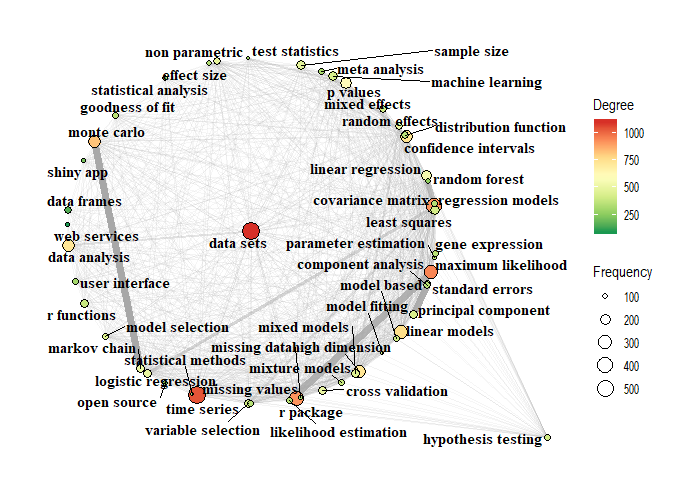
\includegraphics[width=1\linewidth,height=0.3\textheight]{fig5} \caption[Knowledge graph of R based on package description archived on CRAN]{Knowledge graph of R based on package description archived on CRAN. Only the top 50 keywords with the highest frequency are displayed. The width of an edge is proportional to the number of co-occurrences. The graph adopted a radial layout around a focal node wherein the most frequent keyword is selected as the focal node (namely 'data sets' with 539 occurrences). }\label{fig:fig5}
\end{figure}
\end{Schunk}

\hypertarget{collaboration-patterns-in-the-r-community}{%
\subsection{Collaboration patterns in the R
community}\label{collaboration-patterns-in-the-r-community}}

An inspection of the CRAN meta information shows that the number of
authors of a package has a long-tail distribution (Figure 6a). By 2019,
6,645 packages are single-authored, followed by 3,677 with two, 2,227
with three, 1,177 with four, and 599 with five. There are, moreover,
1022 packages written by more than five authors. We see that the number
of authors writing a package is roughly distributed according to Lotka's
square law. This differs with the academic world, where the ubiquity of
teams and the demise of the lone author \citep{WuchtyJones-607}. When a
package has more than one author, we assume that it was written in
collaboration. From this perspective, we found more cooperative works
than single-author ones (8702 v. 6645). Investigating the possible
effects of collaboration (Figure 6b, 6c, 6d), we found a positive
correlation between the number of authors of a package and the number of
imported packages (Pearson, r = 0.16, p \textless{} 2.2e-16), daily
download times (Pearson, r = 0.09, p \textless{} 2.2e-16) and number of
updates per year (Pearson, r = 0.20, p \textless{} 2.2e-16). These
results indicate that the collaborative behavior of R developers might
help to reuse and integrate more sources in the R community and improve
the efficiency of the development of R packages. Moreover, R packages
resulting from teamwork may gain more popularity. This phenomenon is
also common in academia, where collaborative study attracts more
citations than comparable solo research \citep{WuchtyJones-607}.

\begin{Schunk}
\begin{figure}
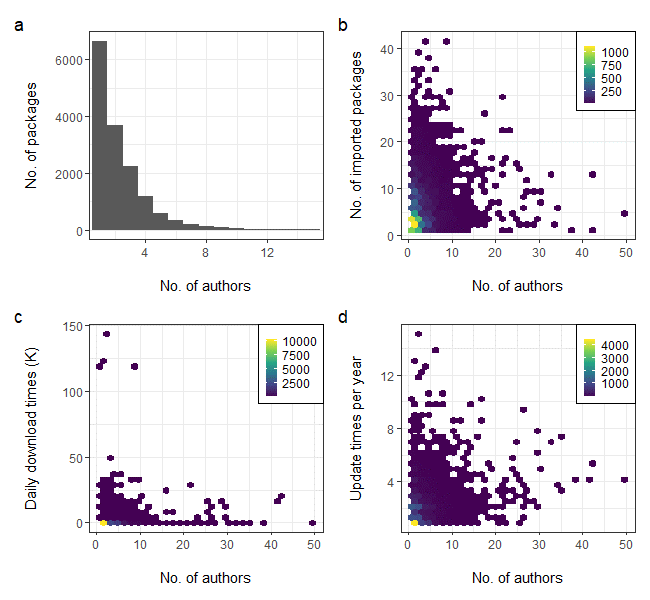
\includegraphics[width=1\linewidth,height=0.3\textheight]{fig6} \caption[Collaboration patterns in R community]{Collaboration patterns in R community. (a) Distribution of the number of authors of R packages (packages with more than 15 authors are omitted). (b) Correlation between the number of authors and the number of imported packages. (c) Correlation between the number of authors and the daily number of downloads. (d) Correlation between the number of authors and the number of updates per year. The legends show how many packages lie in the blocks. }\label{fig:fig6}
\end{figure}
\end{Schunk}

\hypertarget{discussion}{%
\section{Discussion}\label{discussion}}

From the analysis above, we can speculate about the different driving
models (Figure 7) based on the R ecosystem framework (Figure 2) proposed
at the start of this paper. As members from the R ecosystem often hold
more than one roles, we further make abstraction of the roles in the
proposed R ecosystem (software facilities provided by software
developers, statistical tools provided by statistical designers and
real-world problems suggested by general users).

\begin{Schunk}
\begin{figure}
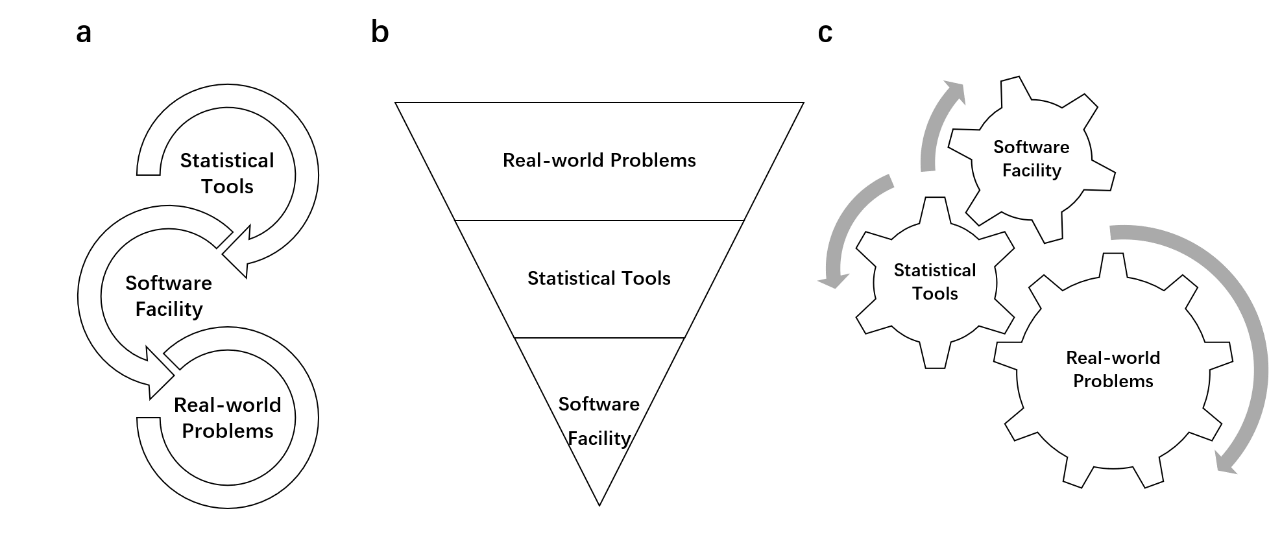
\includegraphics[width=1\linewidth,height=0.3\textheight]{fig7} \caption[The driving models of the R ecosystem from different perspectives]{The driving models of the R ecosystem from different perspectives. (a) From the perspective of statistics. (b) From the perspective of computer science. (c) From the perspective of users. }\label{fig:fig7}
\end{figure}
\end{Schunk}

R was first designed by Ross Ihaka and Robert Gentleman, both
statisticians interested in computer programming, as a personal project
to build statistical tools in a teaching laboratory \citep{Ihaka-500}.
Hence R can be regarded as a fruit of the interplay between statistics
and computer science. Yet, few people would consider R as a serious
programming language, but rather as an environment for statistical
computation. In textbooks of R, students would be taught how to generate
random numbers and draw its distributions, whereas in textbooks of C,
Java, Python, etc., after their ``Hello, World!'' program, they are more
likely to learn different types of data structures and algorithms.
Generally, the development of R is deeply rooted in statistics, a fact
that still can be seen in today's R ecosystem (Figure 5). Usually,
statistical researchers would propose new ideas and implement these
ideas in R, and then test them in the real world (Figure 7a). A
convenient package designed by statisticians provides users with
easy-to-use APIs and tries to guide them to discover more with the help
of additional settings provided by parameters. In this way, even users
without any background knowledge could utilize the cutting-edge
statistical tools in their work. At the same time, they might discover
issues about the usage and give feedback to the package maintainers.
This information then helps them to improve the statistical tools. It is
good practice for developers to keep complete documentation about their
work. We found that the packages with vignette builder have more
downloads than those which have not (11,499 v. 7,073 based on monthly
averages). Moreover, packages with an URL -- providing extra information
- hold a higher number of downloads (13,950 v. 3,223 again based on
monthly averages).

While R is initiated by statistics, recent years have seen a host of
popular packages designed for tasks not directly related to statistics,
such as high-performance computing (\CRANpkg{Rcpp},
\CRANpkg{data.table}, \CRANpkg{doParallel}, etc.), string operations
(\CRANpkg{stringi}, \CRANpkg{stringr}, \CRANpkg{glue}, etc.) and
connection to other software (\CRANpkg{openxlsx}, \CRANpkg{pdftools},
\CRANpkg{sparklyr}, etc.). Generally, these tasks could be categorized
as software facilities, and these facilities have likely acted as
cornerstones supporting the R ecosystem (Figure 7b). According to our
investigation, the usage of R in computer science is relatively
infrequent in academia, but the R packages providing software facilities
are among the most popular ones. As R gets more popular in multiple
fields, developers from different backgrounds are considering building a
more comprehensive ecosystem for it (e.g.~more user-friendly interface
on top and high-performance computing at bottom). Currently, the
light-weighted R software could carry out complicated computations on
million rows of data within minutes, and at the same time storing and
exporting these results to dashboards in expressive graphics and tables.
In the field of data science, the versatile R is not in the least
inferior to Python, which is well-known for its ``glue'' feature. On the
other hand, while there are many statistical tools wrapped in R
packages, end-users might find it difficult to use them directly in
practical applications, because the various application scenarios might
not be considered thoroughly in the early stage of development. Software
facilities, serving as a bridge between statistical tools and real-world
problems, can fill this gap. For instance, some advanced statistical
methods might for the moment only be accessible in R, but the real data
are stored in different file formats (docx, pdf, tiff, json, etc.). Only
by developing file conversion tools can end-users upscale the power of
statistics shared in the community. These tools, serving as software
facilities, are so popular that they may gain more attention than other
specific statistical tools. This is because the functionalities software
facilities provide are considered to be more general and irreplaceable
in the workflow, whereas R provides various alternatives in statistical
methods. In the future, the R community would attract more talents with
a solid computer science background. The sparks between computer science
and statistics could lead to an amazing revolution in the community and
lift the R ecosystem to a higher level.

Although R is rooted in statistics and developed by computer techniques,
the fruit of R is shared on a much broader scale. We found that in
academia, a huge group of researchers from various fields are benefiting
from R. Usually, they start their research from real-world problems,
make hypotheses, and seek the right tools to provide evidence (Figure
7c). These scientific areas are often characterized by embracing the
advent of big data and moving toward evidence-based quantitative
science. In such cases, R has turned out to be one of the most
appropriate tools. In a time in which science emphasizes that academic
results must be reproducible, the documented R scripts provide evidence
for inspection and validation of the whole data science workflow.
Moreover, as the readability of R is rising rapidly, there seems to be a
trend for researchers to communicate and collaborate using R. A
well-designed syntax of the R language could be comprehended by even
non-programmers. Moreover, these codes could also be run effectively and
efficiently in the computer to reproduce the exact same results based on
openly shared data. Not only does R provide researchers with powerful
computational tools to lower the barrier of statistical implementation,
but it also provides an opportunity to facilitate open science through
its design and community culture. This trend could also create a
breeding ground for knowledge transfer and cross-disciplinary research,
as the operational tools (R codes) and statistical logics underneath can
be shared and passed from field to field.

With the joint effort from statisticians, computer scientists and
general users from versatile backgrounds, the ecosystem of R has become
unprecedentedly energetic and diverse in the recent two decades. On CRAN
we can usually find packages with single authors because the open-source
community allows developers to reuse codes freely as long as the license
is not violated. Therefore, when new users start to develop with R and
import functions from other packages, they are standing on the shoulders
of each other already. This feature can be considered an advanced form
of communication and collaboration. Nevertheless, our investigation
shows that there are positive correlations between the number of authors
of packages and the imports, updates, and downloads, which indicates
that teamwork generally improves creativity, developmental efficiency,
and software impact. A large number of local and international R
communities (rOpenSci, RLadies, RStudio, RUGS, etc.), online or offline,
commercial or non-commercial, are emerging and flourishing vigorously
these years. While they have various scopes and organizational forms,
the core spirit of R remains in every one of them, namely to be free,
open, and collaborative, leading to worldwide progress. Therefore, just
forget about the TIOBE Index or the aggressive comparisons with other
programming languages. R is here to stay and there is a bright future to
come.

\hypertarget{acknowledgements}{%
\section{Acknowledgements}\label{acknowledgements}}

The authors thank Ronald Rousseau for useful remarks about their work.

\bibliography{RJreferences.bib}

\address{%
Tian-Yuan Huang\\
National Science Library, Chinese Academy of Sciences\\%
Beijing, China\\
%
%
\textit{ORCiD: \href{https://orcid.org/0000-0002-4151-3764}{0000-0002-4151-3764}}\\%
\href{mailto:huangtianyuan@mail.las.ac.cn}{\nolinkurl{huangtianyuan@mail.las.ac.cn}}%
}

\address{%
Liying Yang\\
National Science Library, Chinese Academy of Sciences\\%
Beijing, China\\
%
%
%
\href{mailto:yangly@mail.las.ac.cn}{\nolinkurl{yangly@mail.las.ac.cn}}%
}
